% Story mode, proposed: one run from the first chapter to the last. A scene
% is won or lost by its objective or its clock; a loss costs a life; with
% none left, the run can continue from the chapter's first scene.
% Standalone: compiles with pdflatex.
\documentclass[tikz,border=4pt]{standalone}
\usetikzlibrary{arrows.meta,positioning,calc,shapes.geometric}

\definecolor{paper}{HTML}{EFE8D8}
\definecolor{ink}{HTML}{2B2A28}
\definecolor{muted}{HTML}{6B6457}
\definecolor{indigo}{HTML}{3E4A89}  % the way forward
\definecolor{ochre}{HTML}{B8862B}   % a loss
\definecolor{ground}{HTML}{D9CDB2}

\newcommand{\Lives}{3}       % lives for a whole run
\newcommand{\SceneMin}{4}    % minutes on each scene's clock
\newcommand{\Step}{3.2}      % vertical step between rows, cm

\begin{document}
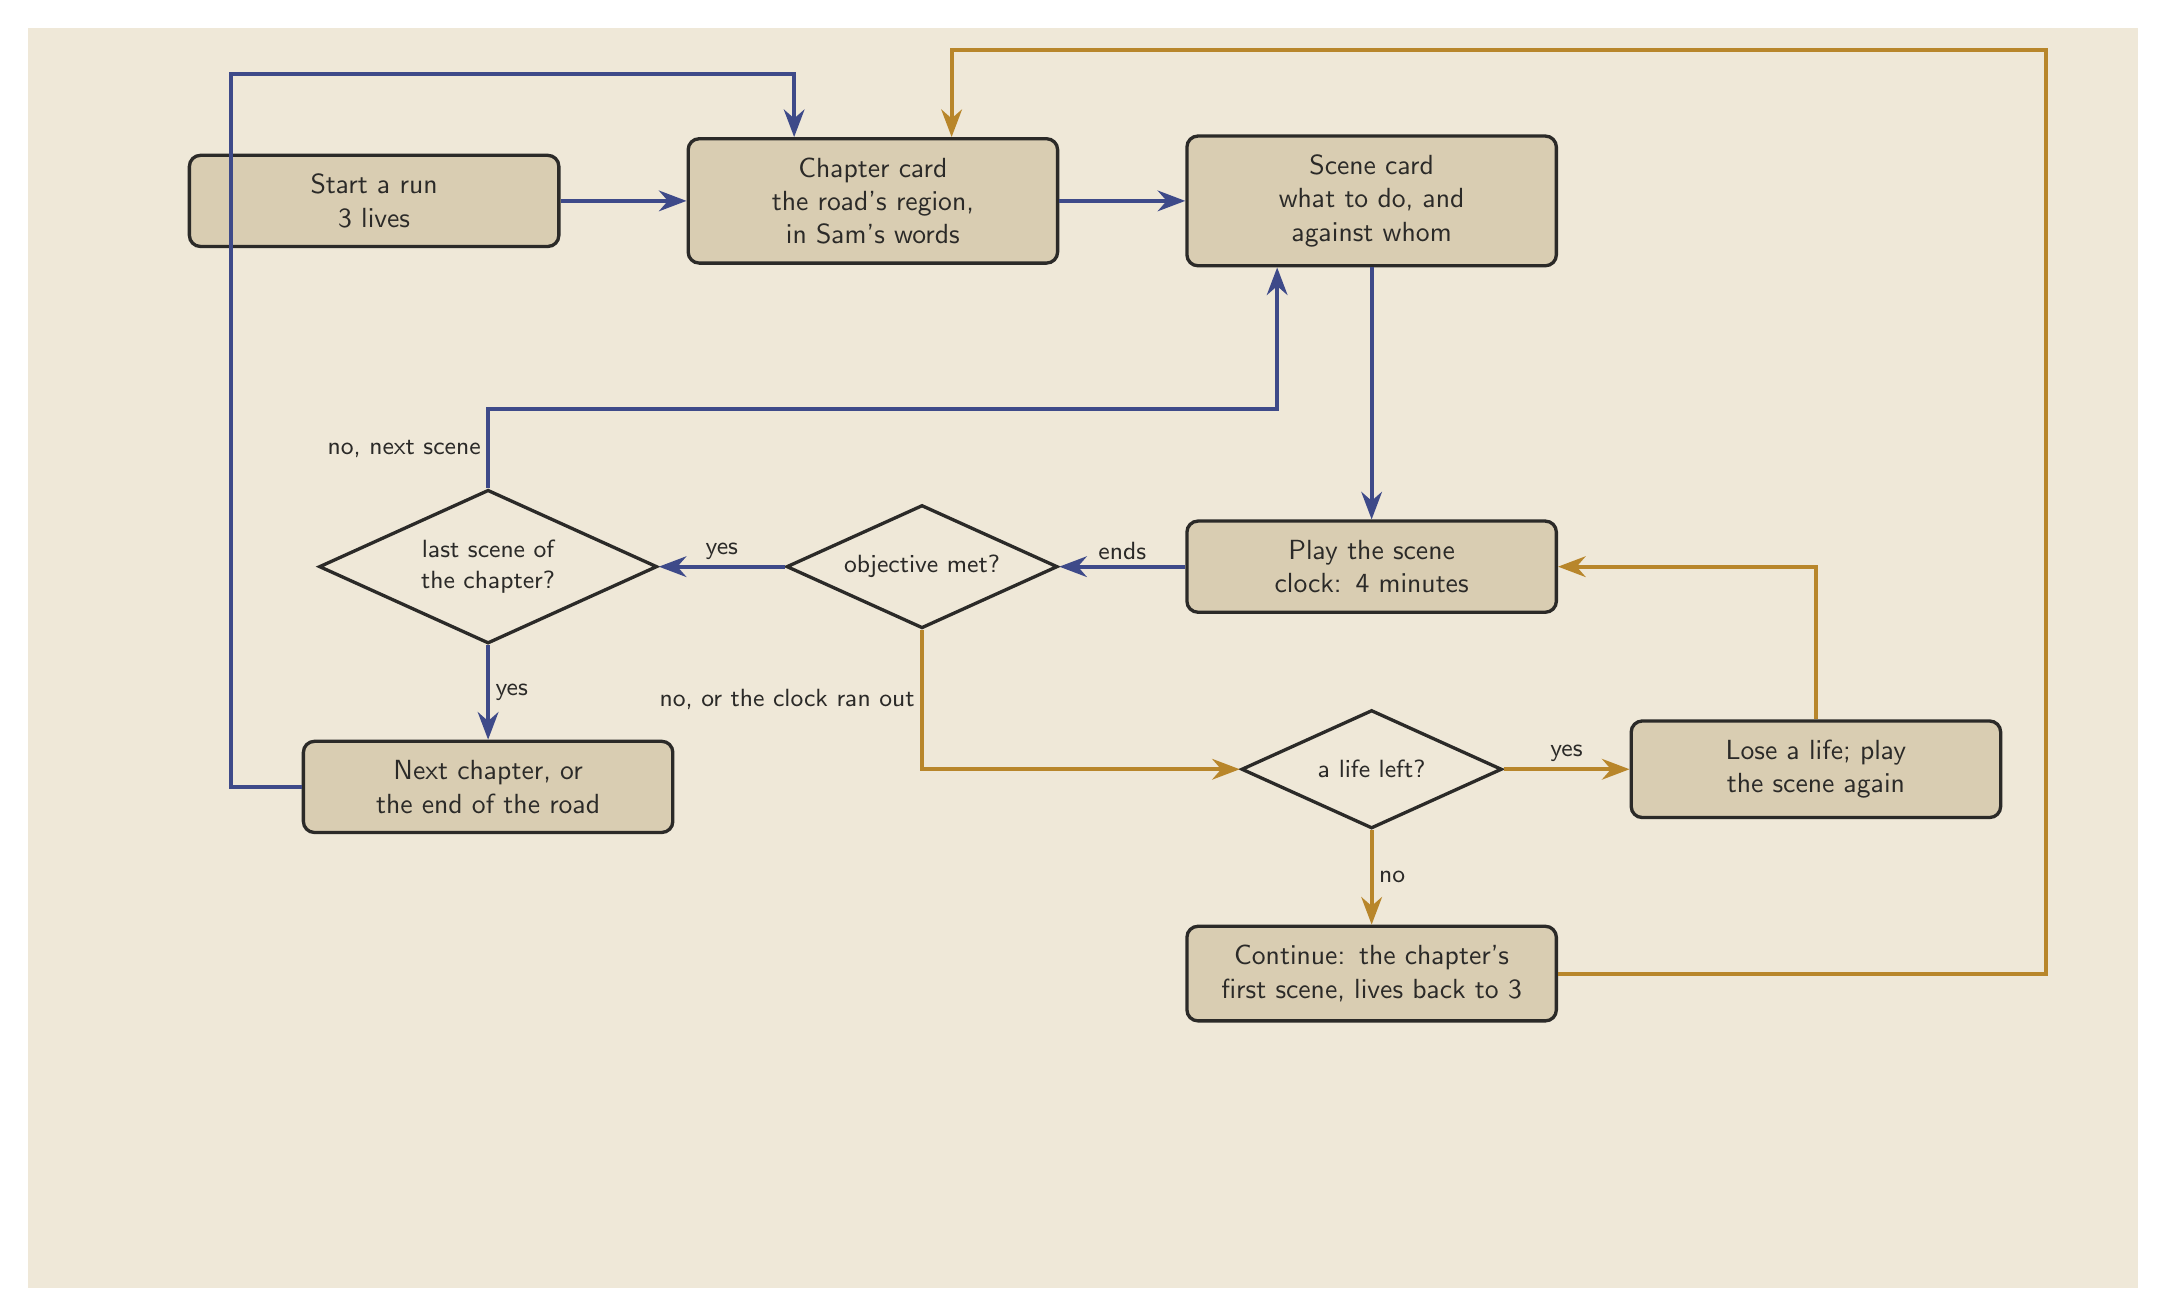
\begin{tikzpicture}[font=\sffamily, ink, node distance=1.2cm and 1.6cm,
    state/.style={draw=ink, line width=1.2pt, fill=ground, rounded corners=4pt, text width=4.2cm, align=center, inner sep=7pt},
    test/.style={draw=ink, line width=1.2pt, fill=paper, diamond, aspect=2.2, text width=2.6cm, align=center, inner sep=1pt, font=\sffamily\small},
    go/.style={-{Stealth[length=3.5mm]}, line width=1.4pt, draw=indigo},
    lose/.style={-{Stealth[length=3.5mm]}, line width=1.4pt, draw=ochre},
    lbl/.style={font=\sffamily\small, fill=paper, inner sep=2pt},
  ]
% --- Background ------------------------------------------------------------------
\fill[paper] (-4.4,2.2) rectangle (22.4,-4*\Step-1.0);

% --- States -------------------------------------------------------------------------
\node[state] (start) at (0,0) {Start a run\\\Lives\ lives};
\node[state, right=of start] (card) {Chapter card\\the road's region, in Sam's words};
\node[state, right=of card] (intro) {Scene card\\what to do, and against whom};
\node[state, below=\Step cm of intro, anchor=north] (play) {Play the scene\\clock: \SceneMin\ minutes};
\node[test, left=of play] (won) {objective met?};
\node[test, left=of won] (more) {last scene of the chapter?};
\node[state, below=of more] (next) {Next chapter, or the end of the road};
\node[test, below=of play] (life) {a life left?};
\node[state, right=of life] (retry) {Lose a life; play the scene again};
\node[state, below=of life] (cont) {Continue: the chapter's first scene, lives back to \Lives};

% --- Arrows (drawn last) -------------------------------------------------------------
% Routes run around the boxes: up the left edge to the chapter card, over the
% top for a continue, and straight down for the next scene.
\draw[go] (start) -- (card);
\draw[go] (card) -- (intro);
\draw[go] (intro) -- (play);
\draw[go] (play) -- node[lbl, above] {ends} (won);
\draw[go] (won) -- node[lbl, above] {yes} (more);
\draw[go] (more.north) -- ++(0,1.0) node[lbl, left, pos=0.5] {no, next scene} -| ($(intro.south)+(-1.2,0)$);
\draw[go] (more) -- node[lbl, right] {yes} (next);
\draw[go] (next.west) -- ++(-0.9,0) |- ($(card.north)+(-1.0,0.8)$) -- ($(card.north)+(-1.0,0)$);
\draw[lose] (won.south) |- node[lbl, pos=0.25, left] {no, or the clock ran out} (life.west);
\draw[lose] (life) -- node[lbl, above] {yes} (retry);
\draw[lose] (retry.north) |- (play.east);
\draw[lose] (life) -- node[lbl, right] {no} (cont);
\draw[lose] (cont.east) -- ++(6.2,0) |- ($(card.north)+(1.0,1.1)$) -- ($(card.north)+(1.0,0)$);
\end{tikzpicture}
\end{document}
